\documentclass{article}
\usepackage[utf8]{inputenc}
\usepackage{graphicx}
\usepackage{fancyhdr}
\usepackage[margin=2cm]{geometry}
\usepackage{array, multirow}
\usepackage{longtable}
\usepackage{amssymb}
\usepackage{enumitem} % For customizing itemize lists
\usepackage{tabularx}
\usepackage{tikz}
\usepackage{dashrule}
\usepackage[most]{tcolorbox}
\usepackage{booktabs}
\usepackage{mdframed}
\usepackage{adjustbox}
\usepackage{pgf-pie} % pie charts
\usepackage{caption}
\usepackage[bottom]{footmisc}
\usepackage[table]{xcolor}
\usepackage{xcolor}
\usepackage{wrapfig}



\title{Technical Edge: Daily Range Expansion Model}
\author{\textbf{MR5OBOT} \\ \small{Mentor \& Concept Credits: Michael J. Huddeston}}
\date{\today}

\begin{document}
\maketitle

\newtcolorbox{notebox}{
    colback=gray!7,
    colframe=gray!0,
    arc=0mm,
    boxrule=0mm,
    left=5mm,
    right=5mm,
    top=1mm,
    bottom=1mm,
}

\renewcommand{\thefootnote}{}
\footnote{Twitter [ @MR-5OBOT ]}
\vspace{0.8cm}

\begin{figure}[h]
  \begin{minipage}{.5\textwidth}
    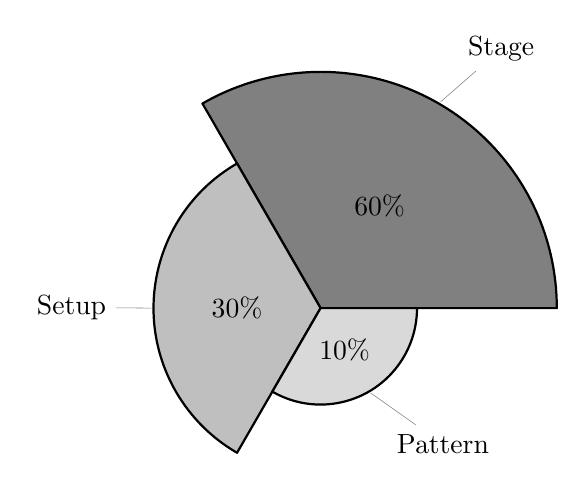
\begin{tikzpicture}[scale=1]
      \pie[polar,text=pin, color={gray!100, gray!50, gray!30}]{60/Stage, 30/Setup, 10/Pattern}
    \end{tikzpicture}
  \end{minipage}
  \begin{minipage}{.45\textwidth}
    \centering
    \section{Model Clarification}
    The following model system is designed to be applied and analyzed in the specific order of : \\
    \vspace{0.5cm}
    HTF = Stage (Bias)\\
    \vspace{0.2cm}
    MTF = Setup (PDA) \\
    \vspace{0.2cm}
    LTF = Pattern (Entry Model)\\
    \vspace{0.2cm}
    \subsection{Model Objective}
    Intraday focus: capturing the obvious SSL/BSL.
  \end{minipage}
\end{figure}
\vspace{1.5cm}


\begin{table}[h!]
\centering
\definecolor{lightgray}{gray}{0.95}
\renewcommand{\arraystretch}{2}
\setlength{\tabcolsep}{30pt}
\rowcolors{2}{lightgray}{}
\begin{tabular}{|c|c|c|}
  \hline
  \multirow{2}{*}{\textbf{STAGE}} & \multirow{2}{*}{\textbf{SETUP}} & \multirow{2}{*}{\textbf{PATTERN}} \\
   & & \\
  \hline
  Daily Range Expansion & \rule{0pt}{60pt}FVG - OB - HIGHs/LOWs\rule[-60pt]{0pt}{0pt} & \-  The Entry Model  \- \\
  \hline
\end{tabular}
% \caption{The Trade Logs}
\end{table}
\newpage

\section{Higher Timeframe}
The stage for the model is based on indentifying the higherst probability direction and draw for the expansion of the daily candle

\vspace{0.6cm}
\begin{figure}[h!]
\begin{minipage}{0.7\textwidth}
\subsection{Identify:}
  \vspace{0.3cm}
  \begin{itemize}
    \item Daily \& Weekly Order flow
    \item Weekly Profiles [day of week]
    \item Daily Profiles [PO3 \& session character]
  \end{itemize}
  \vspace{0.3cm}
$ \rightarrow $ When {\color[HTML]{008000}Bullish,} you are anticipating Open to Low, \\ then expansion toward higher prices \\\\
$ \rightarrow $ When {\color[HTML]{BB5153}Bearish,} you are anticipating Open to High, \\ then expansion towards lower prices
  \vspace{0.3cm}
\subsection{The Context for Expansions}

\end{minipage}

\hfill
\begin{minipage}{0.3\textwidth}
  \includegraphics[scale=0.8]{$HOME/Pictures/latex/OHLC.png}
\end{minipage}
\end{figure}




\newpage
\section{Diagram}

\begin{figure}[h!]
  \caption{London Reversal $\rightarrow$ LHOD}
\begin{adjustbox}{width=1.05\textwidth,center}
  \includegraphics{~/Pictures/latex/LO reversal.png}
\end{adjustbox}
  \label{fig:image}
\end{figure}

\begin{figure}[h!]
  \caption{New York Reversal $\rightarrow$ NHOD}
\begin{adjustbox}{width=1.05\textwidth,center}
  \includegraphics{~/Pictures/latex/NY reversal.png}
\end{adjustbox}
  \label{fig:image}
\end{figure}






\end{document}
